\documentclass{epflreport}%
\usepackage[T1]{fontenc}%
\usepackage[utf8]{inputenc}%
\usepackage{lmodern}%
\usepackage{textcomp}%
\usepackage{lastpage}%
\usepackage{graphicx}%
\usepackage{longtable}%
%
%
%
\begin{document}%
\normalsize%
\frontmatter%
\title{Sheffield two{-}compound study}%
\subtitle{metformin (all results)}%
\author{miblab.org}%
\subject{D2.10 {-} Internal report}%
\affiliation{https://miblab.org}%
\coverimage{cover.jpg}%
\definecolor{title}{HTML}{FF0000}%
\makecover%
\begin{titlepage}%
\begin{center}%
\makeatletter%
\largetitlestyle\fontsize{45}{45}\selectfont\@title%
\makeatother%
\linebreak%
\makeatletter%
\ifdefvoid{\@subtitle}{}{\bigskip\titlestyle\fontsize{20}{20}\selectfont\@subtitle}%
\makeatother%
\linebreak%
\bigskip%
\bigskip%
by%
\linebreak%
\bigskip%
\bigskip%
\makeatletter%
\largetitlestyle\fontsize{25}{25}\selectfont\@author%
\makeatother%
\vfill%
\large%
\begin{tabular}{ll}%
\hline%
Report compiled by: &Steven Sourbron\\%
Institute: &University of Sheffield\\%
Department: &Section of Medical Imaging and Technologies\\%
Email: &s.sourbron@sheffield.ac.uk\\%
Date: &\today\\%
\hline%
\end{tabular}%


\begin{figure}[b!]%
\centering%
\centering%

\includegraphics[width=2in]{C:/Users/md1spsx/Documents/GitHub/tristan-human-modelling/build/metformin/report (complete)_source/layout/tristan-logo.jpg}%
\end{figure}

%
\end{center}%
\end{titlepage}%
\newpage%
\tableofcontents%
\mainmatter%
\clearpage%
\chapter{Two{-}scan results}%
\section{Data summary}%
\label{sec:Datasummary}%

%


\begin{figure}[h!]%
\centering%
\includegraphics[width=7in]{C:/Users/md1spsx/Documents/GitHub/tristan-human-modelling/build/metformin/results (two scans)/Figures/_effect_plot.png}%
\caption{Effect size (\%) on hepatocellular uptake (k\_he, left) and biliary excretion (k\_bh, right) of gadoxetate. The boxplot shows median, interquartile range and 95 percent range. The line plots show individual values for hepatocellular uptake (k\_he, middle) and biliary excretion (k\_bh, right) of gadoxetate of the control (left of plot) and treatment (right of plot). Grey lines are healthy controls with rifampicin injection.}%
\end{figure}

%
\begin{longtable}{rcccccccc}%
\hline%
parameter&count&mean&std&min&25\%&50\%&75\%&max\\%
\hline%
khe effect size (\%)&6.0&{-}7.3&13.2&{-}21.0&{-}15.7&{-}10.8&{-}1.9&14.9\\%
khe control (mL/min/100cm3)&6.0&54.74&9.22&42.6&48.59&54.94&60.55&67.06\\%
khe drug (mL/min/100cm3)&6.0&50.74&10.81&35.96&42.64&53.86&57.68&62.94\\%
kbh effect size (\%)&6.0&11.2&24.2&{-}14.7&{-}8.0&7.6&29.5&43.1\\%
kbh control (mL/min/100cm3)&6.0&2.53&0.98&1.43&1.93&2.18&3.32&3.83\\%
kbh drug (mL/min/100cm3)&6.0&2.78&1.12&1.34&2.04&2.88&3.28&4.44\\%
\hline%
\caption{Effect size and absolute values of hepatocellular uptake (k\_he) and biliary excretion (k\_bh) of gadoxetate} \\%
\end{longtable}%
\clearpage%
\section{Liver biomarkers}%
\label{sec:Liverbiomarkers}%

%
\begin{longtable}{rccc}%
\hline%
Biomarker&p{-}value&Bayes Factor&Odds Ratio\\%
\hline%
AUC for Cl (0{-}35min)&0.76793&0.39&0.77\\%
AUC for Cl (0{-}inf)&0.95528&0.37&1.06\\%
Biliary excretion rate&0.35326&0.56&0.64\\%
Biliary tissue excretion rate&0.7676&0.39&1.17\\%
Extracellular dispersion&0.23017&0.72&4.19\\%
Extracellular mean transit time&0.47682&0.47&2.41\\%
Final biliary excretion rate&0.26405&0.66&0.45\\%
Final hepatocellular uptake rate&0.68796&0.4&1.44\\%
Hematocrit&&&\\%
Hepatocellular mean transit time&0.83026&0.38&0.9\\%
Hepatocellular tissue uptake rate&0.26673&0.66&0.28\\%
Hepatocellular uptake rate&0.24898&0.69&2.06\\%
Initial biliary excretion rate&0.8499&0.38&1.11\\%
Initial hepatocellular uptake rate&0.59543&0.42&1.71\\%
Liver T1{-}MOLLI at 45min&0.49899&0.46&0.65\\%
Liver T1{-}MOLLI at baseline&0.46924&0.48&1.92\\%
Liver T1{-}MOLLI at scan 2&0.37867&0.53&3.57\\%
Liver blood clearance&0.22127&0.74&1.78\\%
Liver extracellular volume fraction&0.05543&1.94&10.6\\%
RE for R1l at 20min&0.88785&0.38&0.89\\%
RE for Sl at 20min&0.63696&0.41&0.69\\%
\hline%
\caption{Results of a pairwise comparison testing for differences in liver biomarkers between control and treatment. The results are ranked by their p-value, with most significant differences at the top of the list.} \\%
\end{longtable}%
\begin{longtable}{rcccc}%
\hline%
Biomarker&Units&control&drug&change (\%)\\%
\hline%
AUC for Cl (0{-}35min)&mM*sec&192.0 (48.0) &199.0 (29.0) &14.3 (35.0) \\%
AUC for Cl (0{-}inf)&mM*sec&681.0 (310.0) &671.0 (120.0) &47.4 (89.0) \\%
Biliary excretion rate&mL/min/100cm3&2.53 (0.79) &2.78 (0.89) &11.2 (19.0) \\%
Biliary tissue excretion rate&mL/min/100cm3&3.35 (0.98) &3.25 (0.84) &{-}0.0278 (19.0) \\%
Extracellular dispersion&\%&74.9 (4.2) &62.5 (17.0) &{-}16.1 (24.0) \\%
Extracellular mean transit time&sec&23.8 (2.6) &20.0 (8.4) &{-}12.6 (41.0) \\%
Final biliary excretion rate&mL/min/100cm3&2.22 (0.54) &2.62 (0.88) &16.6 (24.0) \\%
Final hepatocellular uptake rate&mL/min/100cm3&62.2 (22.0) &57.9 (11.0) &1.59 (24.0) \\%
Hematocrit&\%&45.0 (0.0) &45.0 (0.0) &0.0 (0.0) \\%
Hepatocellular mean transit time&min&33.3 (9.3) &34.0 (9.7) &4.63 (19.0) \\%
Hepatocellular tissue uptake rate&mL/min/100cm3&223.0 (43.0) &598.0 (600.0) &156.0 (240.0) \\%
Hepatocellular uptake rate&mL/min/100cm3&54.7 (7.4) &50.7 (8.6) &{-}7.34 (11.0) \\%
Initial biliary excretion rate&mL/min/100cm3&3.07 (1.4) &2.99 (0.93) &6.3 (29.0) \\%
Initial hepatocellular uptake rate&mL/min/100cm3&47.3 (12.0) &43.6 (6.8) &4.37 (42.0) \\%
Liver T1{-}MOLLI at 45min&sec&0.445 (0.062) &0.47 (0.098) &5.58 (13.0) \\%
Liver T1{-}MOLLI at baseline&sec&0.761 (0.025) &0.75 (0.023) &{-}1.31 (3.5) \\%
Liver T1{-}MOLLI at scan 2&sec&0.621 (0.076) &0.568 (0.041) &{-}5.77 (18.0) \\%
Liver blood clearance&L/min&0.538 (0.11) &0.49 (0.14) &{-}10.4 (12.0) \\%
Liver extracellular volume fraction&mL/100cm3&25.1 (2.6) &16.1 (7.4) &{-}36.3 (27.0) \\%
RE for R1l at 20min&\%&72.0 (24.0) &73.4 (10.0) &27.3 (61.0) \\%
RE for Sl at 20min&\%&61.7 (21.0) &65.8 (9.4) &36.2 (70.0) \\%
\hline%
\caption{Mean values along with their 95 percent confidence intervals for all liver biomarkers of the control and treatment visit. The last column shows the relative change at the treatment visit. The results are ranked by their p-value, with most significant differences at the top of the list.} \\%
\end{longtable}%
\clearpage%
\section{Systemic biomarkers}%
\label{sec:Systemicbiomarkers}%

%
\begin{longtable}{rccc}%
\hline%
Biomarker&p{-}value&Bayes Factor&Odds Ratio\\%
\hline%
AUC for Cb (0{-}35min)&0.31911&0.59&0.4\\%
AUC for Cb (0{-}inf)&0.74479&0.39&0.7\\%
Body extraction fraction&0.81785&0.38&1.36\\%
Cardiac output&0.2283&0.73&1.53\\%
Heart{-}lung dispersion&0.38416&0.53&2.74\\%
Heart{-}lung mean transit time&0.93329&0.37&1.11\\%
Organs blood mean transit time&0.3065&0.6&2.09\\%
Organs extraction fraction&0.08979&1.37&0.28\\%
Organs extravascular mean transit time&0.04821&2.14&8.42\\%
RE for R1b at 20min&0.56233&0.44&0.58\\%
RE for Sb at 20min&0.89265&0.38&1.15\\%
\hline%
\caption{Results of a pairwise comparison testing for differences in systemic biomarkers between control and treatment visit. The results are ranked by their p-value, with most significant differences at the top of the list.} \\%
\end{longtable}%
\begin{longtable}{rcccc}%
\hline%
Biomarker&Units&control&drug&change (\%)\\%
\hline%
AUC for Cb (0{-}35min)&mM*sec&23.6 (6.0) &27.3 (5.9) &26.0 (40.0) \\%
AUC for Cb (0{-}inf)&mM*sec&44.4 (19.0) &48.5 (13.0) &46.0 (83.0) \\%
Body extraction fraction&\%&5.44 (2.2) &5.05 (1.2) &19.4 (54.0) \\%
Cardiac output&L/min&10.5 (3.5) &9.49 (3.2) &{-}9.24 (15.0) \\%
Heart{-}lung dispersion&\%&57.1 (14.0) &48.9 (8.4) &{-}8.09 (23.0) \\%
Heart{-}lung mean transit time&sec&15.0 (4.2) &14.8 (3.7) &9.95 (46.0) \\%
Organs blood mean transit time&sec&32.8 (9.8) &28.1 (8.4) &{-}10.2 (30.0) \\%
Organs extraction fraction&\%&17.2 (2.1) &19.1 (2.3) &11.8 (11.0) \\%
Organs extravascular mean transit time&min&8.02 (0.89) &6.93 (0.57) &{-}12.6 (9.5) \\%
RE for R1b at 20min&\%&14.2 (4.5) &15.7 (3.4) &29.5 (56.0) \\%
RE for Sb at 20min&\%&13.2 (5.1) &12.8 (3.9) &20.5 (67.0) \\%
\hline%
\caption{Mean values along with their 95 percent confidence intervals for all systemic biomarkers at the control and and treatment visit. The last column shows the relative change at the treatment visit. The results are ranked by their p-value, with most significant differences at the top of the list.} \\%
\end{longtable}%
\clearpage%
\section{Comparison to reference values}%
\label{sec:Comparisontoreferencevalues}%

%


\begin{figure}[h!]%
\centering%
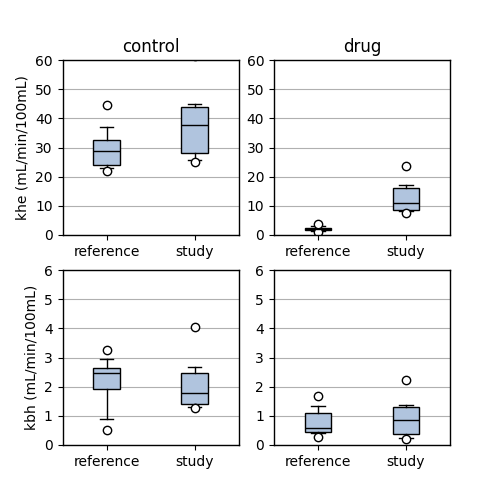
\includegraphics[width=6in]{C:/Users/md1spsx/Documents/GitHub/tristan-human-modelling/build/metformin/results (two scans)/Figures/_compare_to_ref.png}%
\caption{Comparison to reference values in healthy volunteers treated with the drug and under control conditions.}%
\end{figure}

%
\clearpage%
\subsection{Control}%
\label{subsec:Control}%

%
\begin{longtable}{rcccc}%
\hline%
Biomarker&Units&p{-}value&Bayes Factor&Power\\%
\hline%
Hepatocellular uptake rate&mL/min/100cm3&0.00034&302.74&1.0\\%
Liver blood clearance&L/min&0.0035&77.29&1.0\\%
Final hepatocellular uptake rate&mL/min/100cm3&0.02173&4.81&0.87\\%
Extracellular mean transit time&sec&0.04575&2.06&0.38\\%
Liver extracellular volume fraction&mL/100cm3&0.05762&1.68&0.35\\%
Initial hepatocellular uptake rate&mL/min/100cm3&0.07059&1.75&0.64\\%
Liver T1{-}MOLLI at baseline&sec&0.13425&0.97&0.26\\%
Hepatocellular mean transit time&min&0.24708&0.71&0.15\\%
Biliary tissue excretion rate&mL/min/100cm3&0.2742&0.68&0.2\\%
Extracellular dispersion&\%&0.32457&0.62&0.12\\%
Liver T1{-}MOLLI at 45min&sec&0.3835&0.57&0.12\\%
Hepatocellular tissue uptake rate&mL/min/100cm3&0.39344&0.57&0.1\\%
Biliary excretion rate&mL/min/100cm3&0.4813&0.52&0.11\\%
Initial biliary excretion rate&mL/min/100cm3&0.48333&0.52&0.12\\%
RE for R1l at 20min&\%&0.53742&0.5&0.08\\%
Final biliary excretion rate&mL/min/100cm3&0.6057&0.48&0.07\\%
RE for Sl at 20min&\%&0.7892&0.45&0.06\\%
AUC for Cl (0{-}35min)&mM*sec&0.81572&0.44&0.05\\%
AUC for Cl (0{-}inf)&mM*sec&0.8925&0.44&0.05\\%
Liver T1{-}MOLLI at scan 2&sec&0.8927&0.44&0.05\\%
Hematocrit&\%&&&\\%
\hline%
\caption{Results of a pairwise comparison testing for differences in liver biomarkers between this study and healthy reference data, under control conditions.} \\%
\end{longtable}%
\begin{longtable}{rcccc}%
\hline%
Biomarker&Units&p{-}value&Bayes Factor&Power\\%
\hline%
Organs extravascular mean transit time&min&0.01543&3.82&0.61\\%
AUC for Cb (0{-}35min)&mM*sec&0.15453&0.92&0.21\\%
Cardiac output&L/min&0.22484&0.76&0.26\\%
RE for R1b at 20min&\%&0.23558&0.72&0.16\\%
Heart{-}lung dispersion&\%&0.27216&0.68&0.22\\%
Organs blood mean transit time&sec&0.40024&0.57&0.15\\%
Body extraction fraction&\%&0.41498&0.55&0.12\\%
AUC for Cb (0{-}inf)&mM*sec&0.53138&0.5&0.08\\%
Organs extraction fraction&\%&0.55645&0.49&0.08\\%
RE for Sb at 20min&\%&0.69357&0.46&0.06\\%
Heart{-}lung mean transit time&sec&0.84566&0.44&0.05\\%
\hline%
\caption{Results of a pairwise comparison testing for differences in aorta biomarkers between this study and healthy reference data, under control conditions.} \\%
\end{longtable}%
\clearpage%
\subsection{Treatment}%
\label{subsec:Treatment}%

%
\begin{longtable}{rcccc}%
\hline%
Biomarker&Units&p{-}value&Bayes Factor&Power\\%
\hline%
Liver T1{-}MOLLI at scan 2&sec&3e{-}05&650.24&1.0\\%
RE for Sl at 20min&\%&4e{-}05&156700.0&\\%
RE for R1l at 20min&\%&5e{-}05&169400.0&\\%
AUC for Cl (0{-}35min)&mM*sec&6e{-}05&118500.0&1.0\\%
Initial hepatocellular uptake rate&mL/min/100cm3&6e{-}05&145700.0&1.0\\%
Hepatocellular uptake rate&mL/min/100cm3&0.0001&58150.0&\\%
Final hepatocellular uptake rate&mL/min/100cm3&0.00017&20790.0&\\%
AUC for Cl (0{-}inf)&mM*sec&0.00021&8393.48&\\%
Liver blood clearance&L/min&0.00106&711.92&1.0\\%
Biliary tissue excretion rate&mL/min/100cm3&0.00189&43.13&1.0\\%
Extracellular mean transit time&sec&0.00219&17.16&0.95\\%
Liver T1{-}MOLLI at 45min&sec&0.00229&51.28&1.0\\%
Biliary excretion rate&mL/min/100cm3&0.00545&20.86&0.99\\%
Hepatocellular mean transit time&min&0.01166&7.54&0.75\\%
Final biliary excretion rate&mL/min/100cm3&0.03025&2.78&0.69\\%
Liver T1{-}MOLLI at baseline&sec&0.0446&2.0&0.48\\%
Hepatocellular tissue uptake rate&mL/min/100cm3&0.11287&1.35&0.54\\%
Liver extracellular volume fraction&mL/100cm3&0.22882&0.78&0.27\\%
Initial biliary excretion rate&mL/min/100cm3&0.25324&0.72&0.17\\%
Extracellular dispersion&\%&0.41888&0.57&0.15\\%
Hematocrit&\%&&&\\%
\hline%
\caption{Results of a pairwise comparison testing for differences in liver biomarkers between this study and healthy reference data, under treatment conditions.} \\%
\end{longtable}%
\begin{longtable}{rcccc}%
\hline%
Biomarker&Units&p{-}value&Bayes Factor&Power\\%
\hline%
Organs extraction fraction&\%&0.02729&2.66&0.58\\%
RE for R1b at 20min&\%&0.06118&1.62&0.42\\%
Body extraction fraction&\%&0.06201&1.71&0.54\\%
RE for Sb at 20min&\%&0.10917&1.14&0.31\\%
AUC for Cb (0{-}inf)&mM*sec&0.12406&1.04&0.3\\%
AUC for Cb (0{-}35min)&mM*sec&0.14747&0.94&0.27\\%
Cardiac output&L/min&0.33945&0.63&0.19\\%
Organs blood mean transit time&sec&0.63242&0.49&0.07\\%
Organs extravascular mean transit time&min&0.78145&0.46&0.06\\%
Heart{-}lung dispersion&\%&0.81322&0.46&0.06\\%
Heart{-}lung mean transit time&sec&0.90028&0.45&0.05\\%
\hline%
\caption{Results of a pairwise comparison testing for differences in aorta biomarkers between this study and healthy reference data, under treatment conditions.} \\%
\end{longtable}%
\clearpage%
\section{Case notes}%
\label{sec:Casenotes}%

%
\subsection{Subject SHF{-}003}%
\label{subsec:SubjectSHF{-}003}%

%


\begin{figure}[h!]%
\centering%
\includegraphics[width=4.5in]{C:/Users/md1spsx/Documents/GitHub/tristan-human-modelling/build/metformin/results (two scans)/Plots/SHF-003_control.png}%
\caption{Signal{-}time curves for subject SHF{-}003 at the control visit.}%
\end{figure}

%


\begin{figure}[h!]%
\centering%
\includegraphics[width=4.5in]{C:/Users/md1spsx/Documents/GitHub/tristan-human-modelling/build/metformin/results (two scans)/Plots/SHF-003_drug.png}%
\caption{Signal{-}time curves for subject SHF{-}003 at the treatment visit.}%
\end{figure}

%
\clearpage%
\begin{longtable}{rcccc}%
\hline%
Biomarker&Units&control&drug&change (\%)\\%
\hline%
AUC for Cl (0{-}35min)&mM*sec&257.45&199.75&{-}22.41\\%
AUC for Cl (0{-}inf)&mM*sec&1231.06&710.46&{-}42.29\\%
Biliary excretion rate&mL/min/100cm3&1.43&1.34&{-}6.39\\%
Biliary tissue excretion rate&mL/min/100cm3&1.98&1.94&{-}2.1\\%
Extracellular dispersion&\%&75.75&63.14&{-}16.64\\%
Extracellular mean transit time&sec&20.21&19.49&{-}3.55\\%
Final biliary excretion rate&mL/min/100cm3&1.27&1.24&{-}2.56\\%
Final hepatocellular uptake rate&mL/min/100cm3&51.8&41.25&{-}20.36\\%
Hematocrit&\%&45.0&45.0&0.0\\%
Hepatocellular mean transit time&min&50.54&51.63&2.15\\%
Hepatocellular tissue uptake rate&mL/min/100cm3&167.72&126.85&{-}24.37\\%
Hepatocellular uptake rate&mL/min/100cm3&46.52&39.2&{-}15.74\\%
Initial biliary excretion rate&mL/min/100cm3&1.63&1.45&{-}10.86\\%
Initial hepatocellular uptake rate&mL/min/100cm3&41.24&37.14&{-}9.94\\%
Liver T1{-}MOLLI at 45min&sec&0.36&0.39&9.79\\%
Liver T1{-}MOLLI at baseline&sec&0.72&0.76&4.8\\%
Liver T1{-}MOLLI at scan 2&sec&0.47&0.59&26.68\\%
Liver blood clearance&L/min&0.45&0.34&{-}23.31\\%
Liver extracellular volume fraction&mL/100cm3&27.74&30.9&11.41\\%
RE for R1l at 20min&\%&91.79&78.01&{-}15.01\\%
RE for Sl at 20min&\%&79.87&69.67&{-}12.77\\%
\hline%
\caption{Values for liver of subject SHF-003} \\%
\end{longtable}%
\begin{longtable}{rcccc}%
\hline%
Biomarker&Units&control&drug&change (\%)\\%
\hline%
AUC for Cb (0{-}35min)&mM*sec&31.23&26.48&{-}15.21\\%
AUC for Cb (0{-}inf)&mM*sec&62.1&38.43&{-}38.11\\%
Body extraction fraction&\%&3.42&5.85&70.94\\%
Cardiac output&L/min&12.36&12.08&{-}2.26\\%
Heart{-}lung dispersion&\%&84.6&40.47&{-}52.17\\%
Heart{-}lung mean transit time&sec&9.48&19.35&104.08\\%
Organs blood mean transit time&sec&26.38&17.4&{-}34.05\\%
Organs extraction fraction&\%&15.12&17.92&18.54\\%
Organs extravascular mean transit time&min&8.81&6.3&{-}28.44\\%
RE for R1b at 20min&\%&18.1&15.04&{-}16.95\\%
RE for Sb at 20min&\%&20.31&11.57&{-}43.01\\%
\hline%
\caption{Values for aorta of subject SHF-003} \\%
\end{longtable}%
\clearpage%
\subsection{Subject SHF{-}008}%
\label{subsec:SubjectSHF{-}008}%

%


\begin{figure}[h!]%
\centering%
\includegraphics[width=4.5in]{C:/Users/md1spsx/Documents/GitHub/tristan-human-modelling/build/metformin/results (two scans)/Plots/SHF-008_control.png}%
\caption{Signal{-}time curves for subject SHF{-}008 at the control visit.}%
\end{figure}

%


\begin{figure}[h!]%
\centering%
\includegraphics[width=4.5in]{C:/Users/md1spsx/Documents/GitHub/tristan-human-modelling/build/metformin/results (two scans)/Plots/SHF-008_drug.png}%
\caption{Signal{-}time curves for subject SHF{-}008 at the treatment visit.}%
\end{figure}

%
\clearpage%
\begin{longtable}{rcccc}%
\hline%
Biomarker&Units&control&drug&change (\%)\\%
\hline%
AUC for Cl (0{-}35min)&mM*sec&221.89&215.03&{-}3.09\\%
AUC for Cl (0{-}inf)&mM*sec&745.22&774.22&3.89\\%
Biliary excretion rate&mL/min/100cm3&2.06&1.89&{-}8.48\\%
Biliary tissue excretion rate&mL/min/100cm3&2.91&2.2&{-}24.52\\%
Extracellular dispersion&\%&71.38&85.95&20.41\\%
Extracellular mean transit time&sec&22.4&20.82&{-}7.06\\%
Final biliary excretion rate&mL/min/100cm3&2.01&1.87&{-}7.25\\%
Final hepatocellular uptake rate&mL/min/100cm3&32.37&40.37&24.73\\%
Hematocrit&\%&45.0&45.0&0.0\\%
Hepatocellular mean transit time&min&34.38&45.56&32.49\\%
Hepatocellular tissue uptake rate&mL/min/100cm3&146.48&256.76&75.29\\%
Hepatocellular uptake rate&mL/min/100cm3&42.6&35.96&{-}15.58\\%
Initial biliary excretion rate&mL/min/100cm3&2.11&1.91&{-}9.74\\%
Initial hepatocellular uptake rate&mL/min/100cm3&52.83&31.55&{-}40.27\\%
Liver T1{-}MOLLI at 45min&sec&0.42&0.43&1.39\\%
Liver T1{-}MOLLI at baseline&sec&0.79&0.74&{-}5.76\\%
Liver T1{-}MOLLI at scan 2&sec&0.67&0.56&{-}16.31\\%
Liver blood clearance&L/min&0.36&0.28&{-}21.84\\%
Liver extracellular volume fraction&mL/100cm3&29.08&14.01&{-}51.84\\%
RE for R1l at 20min&\%&100.43&81.05&{-}19.29\\%
RE for Sl at 20min&\%&85.95&71.98&{-}16.25\\%
\hline%
\caption{Values for liver of subject SHF-008} \\%
\end{longtable}%
\begin{longtable}{rcccc}%
\hline%
Biomarker&Units&control&drug&change (\%)\\%
\hline%
AUC for Cb (0{-}35min)&mM*sec&27.45&34.7&26.41\\%
AUC for Cb (0{-}inf)&mM*sec&43.95&53.33&21.34\\%
Body extraction fraction&\%&4.29&5.96&38.84\\%
Cardiac output&L/min&7.17&4.26&{-}40.56\\%
Heart{-}lung dispersion&\%&37.19&41.47&11.49\\%
Heart{-}lung mean transit time&sec&11.87&11.2&{-}5.65\\%
Organs blood mean transit time&sec&20.91&32.2&54.0\\%
Organs extraction fraction&\%&15.76&19.42&23.26\\%
Organs extravascular mean transit time&min&6.57&6.35&{-}3.37\\%
RE for R1b at 20min&\%&20.5&18.08&{-}11.79\\%
RE for Sb at 20min&\%&20.61&15.59&{-}24.36\\%
\hline%
\caption{Values for aorta of subject SHF-008} \\%
\end{longtable}%
\clearpage%
\subsection{Subject SHF{-}011}%
\label{subsec:SubjectSHF{-}011}%

%


\begin{figure}[h!]%
\centering%
\includegraphics[width=4.5in]{C:/Users/md1spsx/Documents/GitHub/tristan-human-modelling/build/metformin/results (two scans)/Plots/SHF-011_control.png}%
\caption{Signal{-}time curves for subject SHF{-}011 at the control visit.}%
\end{figure}

%


\begin{figure}[h!]%
\centering%
\includegraphics[width=4.5in]{C:/Users/md1spsx/Documents/GitHub/tristan-human-modelling/build/metformin/results (two scans)/Plots/SHF-011_drug.png}%
\caption{Signal{-}time curves for subject SHF{-}011 at the treatment visit.}%
\end{figure}

%
\clearpage%
\begin{longtable}{rcccc}%
\hline%
Biomarker&Units&control&drug&change (\%)\\%
\hline%
AUC for Cl (0{-}35min)&mM*sec&188.29&249.28&32.4\\%
AUC for Cl (0{-}inf)&mM*sec&307.34&835.63&171.89\\%
Biliary excretion rate&mL/min/100cm3&3.65&4.44&21.57\\%
Biliary tissue excretion rate&mL/min/100cm3&4.91&4.57&{-}6.88\\%
Extracellular dispersion&\%&74.0&21.9&{-}70.41\\%
Extracellular mean transit time&sec&24.99&1.75&{-}92.99\\%
Final biliary excretion rate&mL/min/100cm3&2.67&4.45&66.89\\%
Final hepatocellular uptake rate&mL/min/100cm3&58.91&70.85&20.28\\%
Hematocrit&\%&45.0&45.0&0.0\\%
Hepatocellular mean transit time&min&20.38&21.88&7.39\\%
Hepatocellular tissue uptake rate&mL/min/100cm3&244.29&2110.94&764.11\\%
Hepatocellular uptake rate&mL/min/100cm3&62.37&58.64&{-}5.98\\%
Initial biliary excretion rate&mL/min/100cm3&5.8&4.43&{-}23.58\\%
Initial hepatocellular uptake rate&mL/min/100cm3&65.84&46.44&{-}29.47\\%
Liver T1{-}MOLLI at 45min&sec&0.5&0.42&{-}14.81\\%
Liver T1{-}MOLLI at baseline&sec&0.76&0.72&{-}5.54\\%
Liver T1{-}MOLLI at scan 2&sec&0.71&0.49&{-}30.79\\%
Liver blood clearance&L/min&0.5&0.46&{-}9.68\\%
Liver extracellular volume fraction&mL/100cm3&25.53&2.78&{-}89.12\\%
RE for R1l at 20min&\%&63.32&85.31&34.72\\%
RE for Sl at 20min&\%&53.38&76.77&43.81\\%
\hline%
\caption{Values for liver of subject SHF-011} \\%
\end{longtable}%
\begin{longtable}{rcccc}%
\hline%
Biomarker&Units&control&drug&change (\%)\\%
\hline%
AUC for Cb (0{-}35min)&mM*sec&21.65&35.48&63.85\\%
AUC for Cb (0{-}inf)&mM*sec&28.48&73.96&159.71\\%
Body extraction fraction&\%&7.05&2.43&{-}65.54\\%
Cardiac output&L/min&6.75&7.26&7.52\\%
Heart{-}lung dispersion&\%&49.87&64.61&29.57\\%
Heart{-}lung mean transit time&sec&16.75&7.23&{-}56.84\\%
Organs blood mean transit time&sec&24.14&12.58&{-}47.9\\%
Organs extraction fraction&\%&15.59&15.69&0.61\\%
Organs extravascular mean transit time&min&6.82&7.04&3.13\\%
RE for R1b at 20min&\%&11.47&21.64&88.67\\%
RE for Sb at 20min&\%&11.66&19.1&63.72\\%
\hline%
\caption{Values for aorta of subject SHF-011} \\%
\end{longtable}%
\clearpage%
\subsection{Subject SHF{-}014}%
\label{subsec:SubjectSHF{-}014}%

%


\begin{figure}[h!]%
\centering%
\includegraphics[width=4.5in]{C:/Users/md1spsx/Documents/GitHub/tristan-human-modelling/build/metformin/results (two scans)/Plots/SHF-014_control.png}%
\caption{Signal{-}time curves for subject SHF{-}014 at the control visit.}%
\end{figure}

%


\begin{figure}[h!]%
\centering%
\includegraphics[width=4.5in]{C:/Users/md1spsx/Documents/GitHub/tristan-human-modelling/build/metformin/results (two scans)/Plots/SHF-014_drug.png}%
\caption{Signal{-}time curves for subject SHF{-}014 at the treatment visit.}%
\end{figure}

%
\clearpage%
\begin{longtable}{rcccc}%
\hline%
Biomarker&Units&control&drug&change (\%)\\%
\hline%
AUC for Cl (0{-}35min)&mM*sec&81.01&155.61&92.08\\%
AUC for Cl (0{-}inf)&mM*sec&163.47&497.4&204.28\\%
Biliary excretion rate&mL/min/100cm3&2.3&3.29&43.09\\%
Biliary tissue excretion rate&mL/min/100cm3&3.05&4.07&33.3\\%
Extracellular dispersion&\%&82.02&67.32&{-}17.93\\%
Extracellular mean transit time&sec&20.54&34.32&67.14\\%
Final biliary excretion rate&mL/min/100cm3&2.17&2.89&33.33\\%
Final hepatocellular uptake rate&mL/min/100cm3&112.77&62.16&{-}44.88\\%
Hematocrit&\%&45.0&45.0&0.0\\%
Hepatocellular mean transit time&min&32.74&24.56&{-}24.98\\%
Hepatocellular tissue uptake rate&mL/min/100cm3&270.86&275.26&1.63\\%
Hepatocellular uptake rate&mL/min/100cm3&67.06&52.95&{-}21.04\\%
Initial biliary excretion rate&mL/min/100cm3&2.44&3.81&55.93\\%
Initial hepatocellular uptake rate&mL/min/100cm3&21.34&43.73&104.89\\%
Liver T1{-}MOLLI at 45min&sec&0.56&0.72&29.04\\%
Liver T1{-}MOLLI at baseline&sec&0.73&0.72&{-}1.47\\%
Liver T1{-}MOLLI at scan 2&sec&0.69&0.56&{-}19.85\\%
Liver blood clearance&L/min&0.75&0.62&{-}16.9\\%
Liver extracellular volume fraction&mL/100cm3&24.76&19.23&{-}22.31\\%
RE for R1l at 20min&\%&18.91&52.24&176.22\\%
RE for Sl at 20min&\%&14.92&45.69&206.31\\%
\hline%
\caption{Values for liver of subject SHF-014} \\%
\end{longtable}%
\begin{longtable}{rcccc}%
\hline%
Biomarker&Units&control&drug&change (\%)\\%
\hline%
AUC for Cb (0{-}35min)&mM*sec&10.79&22.18&105.55\\%
AUC for Cb (0{-}inf)&mM*sec&14.87&43.51&192.65\\%
Body extraction fraction&\%&10.16&4.16&{-}59.1\\%
Cardiac output&L/min&17.97&14.57&{-}18.91\\%
Heart{-}lung dispersion&\%&56.36&57.21&1.49\\%
Heart{-}lung mean transit time&sec&24.5&16.09&{-}34.35\\%
Organs blood mean transit time&sec&49.11&34.69&{-}29.36\\%
Organs extraction fraction&\%&18.44&17.15&{-}7.0\\%
Organs extravascular mean transit time&min&8.83&8.11&{-}8.1\\%
RE for R1b at 20min&\%&5.38&13.14&144.34\\%
RE for Sb at 20min&\%&5.76&15.59&170.45\\%
\hline%
\caption{Values for aorta of subject SHF-014} \\%
\end{longtable}%
\clearpage%
\subsection{Subject SHF{-}021}%
\label{subsec:SubjectSHF{-}021}%

%


\begin{figure}[h!]%
\centering%
\includegraphics[width=4.5in]{C:/Users/md1spsx/Documents/GitHub/tristan-human-modelling/build/metformin/results (two scans)/Plots/SHF-021_control.png}%
\caption{Signal{-}time curves for subject SHF{-}021 at the control visit.}%
\end{figure}

%


\begin{figure}[h!]%
\centering%
\includegraphics[width=4.5in]{C:/Users/md1spsx/Documents/GitHub/tristan-human-modelling/build/metformin/results (two scans)/Plots/SHF-021_drug.png}%
\caption{Signal{-}time curves for subject SHF{-}021 at the treatment visit.}%
\end{figure}

%
\clearpage%
\begin{longtable}{rcccc}%
\hline%
Biomarker&Units&control&drug&change (\%)\\%
\hline%
AUC for Cl (0{-}35min)&mM*sec&196.44&215.64&9.78\\%
AUC for Cl (0{-}inf)&mM*sec&846.18&737.5&{-}12.84\\%
Biliary excretion rate&mL/min/100cm3&3.83&3.26&{-}14.72\\%
Biliary tissue excretion rate&mL/min/100cm3&4.79&3.7&{-}22.59\\%
Extracellular dispersion&\%&67.39&65.95&{-}2.14\\%
Extracellular mean transit time&sec&28.16&20.19&{-}28.3\\%
Final biliary excretion rate&mL/min/100cm3&3.26&2.95&{-}9.46\\%
Final hepatocellular uptake rate&mL/min/100cm3&64.59&62.85&{-}2.7\\%
Hematocrit&\%&45.0&45.0&0.0\\%
Hepatocellular mean transit time&min&20.9&26.99&29.18\\%
Hepatocellular tissue uptake rate&mL/min/100cm3&275.07&460.55&67.43\\%
Hepatocellular uptake rate&mL/min/100cm3&55.08&54.78&{-}0.55\\%
Initial biliary excretion rate&mL/min/100cm3&4.63&3.65&{-}21.21\\%
Initial hepatocellular uptake rate&mL/min/100cm3&45.57&46.71&2.5\\%
Liver T1{-}MOLLI at 45min&sec&0.47&0.43&{-}8.89\\%
Liver T1{-}MOLLI at baseline&sec&0.8&0.78&{-}2.93\\%
Liver T1{-}MOLLI at scan 2&sec&0.64&0.56&{-}12.25\\%
Liver blood clearance&L/min&0.54&0.49&{-}8.85\\%
Liver extracellular volume fraction&mL/100cm3&20.02&11.89&{-}40.6\\%
RE for R1l at 20min&\%&70.04&80.28&14.63\\%
RE for Sl at 20min&\%&62.14&73.04&17.54\\%
\hline%
\caption{Values for liver of subject SHF-021} \\%
\end{longtable}%
\begin{longtable}{rcccc}%
\hline%
Biomarker&Units&control&drug&change (\%)\\%
\hline%
AUC for Cb (0{-}35min)&mM*sec&29.36&28.68&{-}2.33\\%
AUC for Cb (0{-}inf)&mM*sec&81.84&56.41&{-}31.06\\%
Body extraction fraction&\%&2.63&5.21&98.56\\%
Cardiac output&L/min&7.26&6.7&{-}7.75\\%
Heart{-}lung dispersion&\%&71.75&50.95&{-}28.99\\%
Heart{-}lung mean transit time&sec&13.29&18.64&40.26\\%
Organs blood mean transit time&sec&47.32&39.06&{-}17.46\\%
Organs extraction fraction&\%&22.02&23.6&7.17\\%
Organs extravascular mean transit time&min&9.17&7.34&{-}19.98\\%
RE for R1b at 20min&\%&17.56&16.75&{-}4.63\\%
RE for Sb at 20min&\%&7.03&7.09&0.96\\%
\hline%
\caption{Values for aorta of subject SHF-021} \\%
\end{longtable}%
\clearpage%
\subsection{Subject SHF{-}022}%
\label{subsec:SubjectSHF{-}022}%

%


\begin{figure}[h!]%
\centering%
\includegraphics[width=4.5in]{C:/Users/md1spsx/Documents/GitHub/tristan-human-modelling/build/metformin/results (two scans)/Plots/SHF-022_control.png}%
\caption{Signal{-}time curves for subject SHF{-}022 at the control visit.}%
\end{figure}

%


\begin{figure}[h!]%
\centering%
\includegraphics[width=4.5in]{C:/Users/md1spsx/Documents/GitHub/tristan-human-modelling/build/metformin/results (two scans)/Plots/SHF-022_drug.png}%
\caption{Signal{-}time curves for subject SHF{-}022 at the treatment visit.}%
\end{figure}

%
\clearpage%
\begin{longtable}{rcccc}%
\hline%
Biomarker&Units&control&drug&change (\%)\\%
\hline%
AUC for Cl (0{-}35min)&mM*sec&209.83&161.5&{-}23.03\\%
AUC for Cl (0{-}inf)&mM*sec&791.04&472.25&{-}40.3\\%
Biliary excretion rate&mL/min/100cm3&1.88&2.49&32.09\\%
Biliary tissue excretion rate&mL/min/100cm3&2.46&3.02&22.63\\%
Extracellular dispersion&\%&78.72&70.94&{-}9.89\\%
Extracellular mean transit time&sec&26.31&23.44&{-}10.91\\%
Final biliary excretion rate&mL/min/100cm3&1.96&2.33&18.87\\%
Final hepatocellular uptake rate&mL/min/100cm3&52.74&69.86&32.48\\%
Hematocrit&\%&45.0&45.0&0.0\\%
Hepatocellular mean transit time&min&40.65&33.15&{-}18.45\\%
Hepatocellular tissue uptake rate&mL/min/100cm3&233.65&358.7&53.52\\%
Hepatocellular uptake rate&mL/min/100cm3&54.8&62.94&14.85\\%
Initial biliary excretion rate&mL/min/100cm3&1.81&2.67&47.27\\%
Initial hepatocellular uptake rate&mL/min/100cm3&56.86&56.01&{-}1.49\\%
Liver T1{-}MOLLI at 45min&sec&0.37&0.43&16.95\\%
Liver T1{-}MOLLI at baseline&sec&0.76&0.78&3.03\\%
Liver T1{-}MOLLI at scan 2&sec&0.55&0.65&17.9\\%
Liver blood clearance&L/min&0.62&0.74&18.32\\%
Liver extracellular volume fraction&mL/100cm3&23.45&17.55&{-}25.19\\%
RE for R1l at 20min&\%&87.22&63.45&{-}27.26\\%
RE for Sl at 20min&\%&73.81&57.89&{-}21.57\\%
\hline%
\caption{Values for liver of subject SHF-022} \\%
\end{longtable}%
\begin{longtable}{rcccc}%
\hline%
Biomarker&Units&control&drug&change (\%)\\%
\hline%
AUC for Cb (0{-}35min)&mM*sec&21.23&16.45&{-}22.55\\%
AUC for Cb (0{-}inf)&mM*sec&35.15&25.11&{-}28.55\\%
Body extraction fraction&\%&5.06&6.71&32.64\\%
Cardiac output&L/min&11.35&12.09&6.53\\%
Heart{-}lung dispersion&\%&42.66&38.42&{-}9.95\\%
Heart{-}lung mean transit time&sec&14.3&16.04&12.21\\%
Organs blood mean transit time&sec&28.66&32.62&13.82\\%
Organs extraction fraction&\%&16.34&20.95&28.25\\%
Organs extravascular mean transit time&min&7.95&6.43&{-}19.11\\%
RE for R1b at 20min&\%&12.01&9.32&{-}22.39\\%
RE for Sb at 20min&\%&13.82&7.6&{-}45.02\\%
\hline%
\caption{Values for aorta of subject SHF-022} \\%
\end{longtable}%
\clearpage%
\chapter{One{-}scan results}%
\section{Data summary}%
\label{sec:Datasummary}%

%


\begin{figure}[h!]%
\centering%
\includegraphics[width=7in]{C:/Users/md1spsx/Documents/GitHub/tristan-human-modelling/build/metformin/results (one scan)/Figures/_effect_plot.png}%
\caption{Effect size (\%) on hepatocellular uptake (k\_he, left) and biliary excretion (k\_bh, right) of gadoxetate. The boxplot shows median, interquartile range and 95 percent range. The line plots show individual values for hepatocellular uptake (k\_he, middle) and biliary excretion (k\_bh, right) of gadoxetate of the control (left of plot) and treatment (right of plot). Grey lines are healthy controls with rifampicin injection.}%
\end{figure}

%
\begin{longtable}{rcccccccc}%
\hline%
parameter&count&mean&std&min&25\%&50\%&75\%&max\\%
\hline%
khe effect size (\%)&6.0&{-}2.2&26.3&{-}35.2&{-}20.7&{-}1.2&10.5&37.2\\%
khe control (mL/min/100cm3)&6.0&46.34&9.87&32.62&41.0&45.84&51.72&60.66\\%
khe drug (mL/min/100cm3)&6.0&44.06&10.01&30.6&38.09&45.35&47.34&59.38\\%
kbh effect size (\%)&6.0&13.3&31.4&{-}10.7&{-}5.7&1.5&17.4&72.9\\%
kbh control (mL/min/100cm3)&6.0&2.51&1.25&1.3&1.67&2.01&3.44&4.24\\%
kbh drug (mL/min/100cm3)&6.0&2.7&1.05&1.3&1.86&2.94&3.54&3.79\\%
\hline%
\caption{Effect size and absolute values of hepatocellular uptake (k\_he) and biliary excretion (k\_bh) of gadoxetate} \\%
\end{longtable}%
\clearpage%
\section{Liver biomarkers}%
\label{sec:Liverbiomarkers}%

%
\begin{longtable}{rccc}%
\hline%
Biomarker&p{-}value&Bayes Factor&Odds Ratio\\%
\hline%
AUC for Cl (0{-}35min)&0.86209&0.38&0.86\\%
AUC for Cl (0{-}inf)&0.80839&0.38&1.29\\%
Biliary excretion rate&0.50816&0.46&0.74\\%
Biliary tissue excretion rate&0.91801&0.38&1.06\\%
Extracellular dispersion&0.58153&0.43&1.82\\%
Extracellular mean transit time&0.17297&0.87&0.24\\%
Hematocrit&&&\\%
Hepatocellular mean transit time&0.66415&0.41&1.24\\%
Hepatocellular tissue uptake rate&0.87198&0.38&0.86\\%
Hepatocellular uptake rate&0.65042&0.41&1.52\\%
Liver T1{-}MOLLI at 45min&0.49899&0.46&0.65\\%
Liver T1{-}MOLLI at baseline&0.46924&0.48&1.92\\%
Liver blood clearance&0.71944&0.4&1.31\\%
Liver extracellular volume fraction&0.44276&0.49&2.45\\%
RE for R1l at 20min&0.89461&0.38&0.9\\%
RE for Sl at 20min&0.80594&0.38&0.8\\%
\hline%
\caption{Results of a pairwise comparison testing for differences in liver biomarkers between control and treatment. The results are ranked by their p-value, with most significant differences at the top of the list.} \\%
\end{longtable}%
\begin{longtable}{rcccc}%
\hline%
Biomarker&Units&control&drug&change (\%)\\%
\hline%
AUC for Cl (0{-}35min)&mM*sec&181.0 (57.0) &186.0 (26.0) &25.9 (58.0) \\%
AUC for Cl (0{-}inf)&mM*sec&774.0 (370.0) &727.0 (100.0) &49.5 (100.0) \\%
Biliary excretion rate&mL/min/100cm3&2.51 (1.0) &2.7 (0.84) &13.3 (25.0) \\%
Biliary tissue excretion rate&mL/min/100cm3&3.57 (1.4) &3.52 (0.97) &6.09 (24.0) \\%
Extracellular dispersion&\%&85.5 (7.8) &82.0 (9.3) &{-}3.2 (13.0) \\%
Extracellular mean transit time&sec&33.4 (11.0) &43.1 (8.5) &39.6 (35.0) \\%
Hematocrit&\%&45.0 (0.0) &45.0 (0.0) &0.0 (0.0) \\%
Hepatocellular mean transit time&min&33.8 (12.0) &32.1 (11.0) &0.599 (22.0) \\%
Hepatocellular tissue uptake rate&mL/min/100cm3&194.0 (95.0) &202.0 (71.0) &26.6 (55.0) \\%
Hepatocellular uptake rate&mL/min/100cm3&46.3 (7.9) &44.1 (8.0) &{-}2.2 (21.0) \\%
Liver T1{-}MOLLI at 45min&sec&0.445 (0.062) &0.47 (0.098) &5.58 (13.0) \\%
Liver T1{-}MOLLI at baseline&sec&0.761 (0.025) &0.75 (0.023) &{-}1.31 (3.5) \\%
Liver blood clearance&L/min&0.447 (0.072) &0.428 (0.13) &{-}4.58 (25.0) \\%
Liver extracellular volume fraction&mL/100cm3&29.1 (8.9) &24.3 (6.7) &{-}0.278 (54.0) \\%
RE for R1l at 20min&\%&72.8 (23.0) &74.1 (10.0) &25.3 (57.0) \\%
RE for Sl at 20min&\%&62.7 (21.0) &65.2 (7.9) &35.9 (76.0) \\%
\hline%
\caption{Mean values along with their 95 percent confidence intervals for all liver biomarkers of the control and treatment visit. The last column shows the relative change at the treatment visit. The results are ranked by their p-value, with most significant differences at the top of the list.} \\%
\end{longtable}%
\clearpage%
\section{Systemic biomarkers}%
\label{sec:Systemicbiomarkers}%

%
\begin{longtable}{rccc}%
\hline%
Biomarker&p{-}value&Bayes Factor&Odds Ratio\\%
\hline%
AUC for Cb (0{-}35min)&0.27329&0.65&0.36\\%
AUC for Cb (0{-}inf)&0.61377&0.42&0.58\\%
Body extraction fraction&0.73864&0.39&1.54\\%
Cardiac output&0.37728&0.54&1.59\\%
Heart{-}lung dispersion&0.04297&2.33&0.28\\%
Heart{-}lung mean transit time&0.32374&0.58&3.45\\%
Organs blood mean transit time&0.62147&0.42&0.67\\%
Organs extraction fraction&0.86332&0.38&1.23\\%
Organs extravascular mean transit time&0.54396&0.44&2.41\\%
RE for R1b at 20min&0.42167&0.5&0.45\\%
RE for Sb at 20min&0.96614&0.37&0.95\\%
\hline%
\caption{Results of a pairwise comparison testing for differences in systemic biomarkers between control and treatment visit. The results are ranked by their p-value, with most significant differences at the top of the list.} \\%
\end{longtable}%
\begin{longtable}{rcccc}%
\hline%
Biomarker&Units&control&drug&change (\%)\\%
\hline%
AUC for Cb (0{-}35min)&mM*sec&24.1 (6.4) &28.6 (6.2) &32.8 (49.0) \\%
AUC for Cb (0{-}inf)&mM*sec&51.9 (21.0) &58.6 (15.0) &56.4 (100.0) \\%
Body extraction fraction&\%&4.96 (2.2) &4.44 (1.0) &12.1 (43.0) \\%
Cardiac output&L/min&9.57 (3.4) &8.49 (3.3) &{-}11.2 (25.0) \\%
Heart{-}lung dispersion&\%&54.1 (17.0) &67.3 (13.0) &30.3 (23.0) \\%
Heart{-}lung mean transit time&sec&19.6 (4.9) &16.0 (3.5) &{-}10.9 (34.0) \\%
Organs blood mean transit time&sec&33.9 (12.0) &36.6 (7.4) &22.2 (40.0) \\%
Organs extraction fraction&\%&24.1 (11.0) &22.9 (3.7) &16.2 (44.0) \\%
Organs extravascular mean transit time&min&8.12 (2.9) &6.77 (1.3) &42.1 (140.0) \\%
RE for R1b at 20min&\%&14.6 (4.4) &16.9 (3.8) &32.8 (54.0) \\%
RE for Sb at 20min&\%&15.2 (8.1) &15.4 (3.1) &48.0 (81.0) \\%
\hline%
\caption{Mean values along with their 95 percent confidence intervals for all systemic biomarkers at the control and and treatment visit. The last column shows the relative change at the treatment visit. The results are ranked by their p-value, with most significant differences at the top of the list.} \\%
\end{longtable}%
\clearpage%
\section{Case notes}%
\label{sec:Casenotes}%

%
\subsection{Subject SHF{-}003}%
\label{subsec:SubjectSHF{-}003}%

%


\begin{figure}[h!]%
\centering%
\includegraphics[width=4.5in]{C:/Users/md1spsx/Documents/GitHub/tristan-human-modelling/build/metformin/results (one scan)/Plots/SHF-003_control.png}%
\caption{Signal{-}time curves for subject SHF{-}003 at the control visit.}%
\end{figure}

%


\begin{figure}[h!]%
\centering%
\includegraphics[width=4.5in]{C:/Users/md1spsx/Documents/GitHub/tristan-human-modelling/build/metformin/results (one scan)/Plots/SHF-003_drug.png}%
\caption{Signal{-}time curves for subject SHF{-}003 at the treatment visit.}%
\end{figure}

%
\clearpage%
\begin{longtable}{rcccc}%
\hline%
Biomarker&Units&control&drug&change (\%)\\%
\hline%
AUC for Cl (0{-}35min)&mM*sec&243.36&197.49&{-}18.85\\%
AUC for Cl (0{-}inf)&mM*sec&1483.62&758.31&{-}48.89\\%
Biliary excretion rate&mL/min/100cm3&1.3&1.3&{-}0.57\\%
Biliary tissue excretion rate&mL/min/100cm3&1.81&2.08&14.45\\%
Extracellular dispersion&\%&82.13&87.0&5.93\\%
Extracellular mean transit time&sec&24.28&39.76&63.74\\%
Hematocrit&\%&45.0&45.0&0.0\\%
Hepatocellular mean transit time&min&55.14&48.18&{-}12.63\\%
Hepatocellular tissue uptake rate&mL/min/100cm3&141.92&95.62&{-}32.62\\%
Hepatocellular uptake rate&mL/min/100cm3&39.84&35.87&{-}9.96\\%
Liver T1{-}MOLLI at 45min&sec&0.36&0.39&9.79\\%
Liver T1{-}MOLLI at baseline&sec&0.72&0.76&4.8\\%
Liver blood clearance&L/min&0.38&0.31&{-}18.05\\%
Liver extracellular volume fraction&mL/100cm3&28.07&37.51&33.63\\%
RE for R1l at 20min&\%&93.17&79.19&{-}15.0\\%
RE for Sl at 20min&\%&85.61&67.73&{-}20.88\\%
\hline%
\caption{Values for liver of subject SHF-003} \\%
\end{longtable}%
\begin{longtable}{rcccc}%
\hline%
Biomarker&Units&control&drug&change (\%)\\%
\hline%
AUC for Cb (0{-}35min)&mM*sec&31.94&28.49&{-}10.8\\%
AUC for Cb (0{-}inf)&mM*sec&78.68&44.66&{-}43.24\\%
Body extraction fraction&\%&2.91&5.38&85.06\\%
Cardiac output&L/min&10.12&11.26&11.3\\%
Heart{-}lung dispersion&\%&61.64&78.81&27.85\\%
Heart{-}lung mean transit time&sec&18.08&9.97&{-}44.84\\%
Organs blood mean transit time&sec&29.8&32.42&8.77\\%
Organs extraction fraction&\%&17.32&18.66&7.77\\%
Organs extravascular mean transit time&min&10.83&6.2&{-}42.79\\%
RE for R1b at 20min&\%&18.42&16.56&{-}10.1\\%
RE for Sb at 20min&\%&20.51&14.52&{-}29.19\\%
\hline%
\caption{Values for aorta of subject SHF-003} \\%
\end{longtable}%
\clearpage%
\subsection{Subject SHF{-}008}%
\label{subsec:SubjectSHF{-}008}%

%


\begin{figure}[h!]%
\centering%
\includegraphics[width=4.5in]{C:/Users/md1spsx/Documents/GitHub/tristan-human-modelling/build/metformin/results (one scan)/Plots/SHF-008_control.png}%
\caption{Signal{-}time curves for subject SHF{-}008 at the control visit.}%
\end{figure}

%


\begin{figure}[h!]%
\centering%
\includegraphics[width=4.5in]{C:/Users/md1spsx/Documents/GitHub/tristan-human-modelling/build/metformin/results (one scan)/Plots/SHF-008_drug.png}%
\caption{Signal{-}time curves for subject SHF{-}008 at the treatment visit.}%
\end{figure}

%
\clearpage%
\begin{longtable}{rcccc}%
\hline%
Biomarker&Units&control&drug&change (\%)\\%
\hline%
AUC for Cl (0{-}35min)&mM*sec&241.82&204.67&{-}15.37\\%
AUC for Cl (0{-}inf)&mM*sec&883.79&790.64&{-}10.54\\%
Biliary excretion rate&mL/min/100cm3&1.58&1.63&3.61\\%
Biliary tissue excretion rate&mL/min/100cm3&2.47&2.02&{-}18.13\\%
Extracellular dispersion&\%&86.81&87.09&0.33\\%
Extracellular mean transit time&sec&25.01&37.16&48.61\\%
Hematocrit&\%&45.0&45.0&0.0\\%
Hepatocellular mean transit time&min&40.44&49.4&22.15\\%
Hepatocellular tissue uptake rate&mL/min/100cm3&130.08&158.07&21.52\\%
Hepatocellular uptake rate&mL/min/100cm3&47.19&30.6&{-}35.17\\%
Liver T1{-}MOLLI at 45min&sec&0.42&0.43&1.39\\%
Liver T1{-}MOLLI at baseline&sec&0.79&0.74&{-}5.76\\%
Liver blood clearance&L/min&0.4&0.24&{-}39.98\\%
Liver extracellular volume fraction&mL/100cm3&36.28&19.36&{-}46.65\\%
RE for R1l at 20min&\%&101.1&81.59&{-}19.3\\%
RE for Sl at 20min&\%&83.08&70.63&{-}14.98\\%
\hline%
\caption{Values for liver of subject SHF-008} \\%
\end{longtable}%
\begin{longtable}{rcccc}%
\hline%
Biomarker&Units&control&drug&change (\%)\\%
\hline%
AUC for Cb (0{-}35min)&mM*sec&28.07&35.83&27.61\\%
AUC for Cb (0{-}inf)&mM*sec&46.6&54.09&16.07\\%
Body extraction fraction&\%&4.07&5.86&44.03\\%
Cardiac output&L/min&7.1&4.28&{-}39.66\\%
Heart{-}lung dispersion&\%&30.66&36.08&17.7\\%
Heart{-}lung mean transit time&sec&15.39&15.96&3.67\\%
Organs blood mean transit time&sec&15.1&30.41&101.31\\%
Organs extraction fraction&\%&14.9&19.65&31.82\\%
Organs extravascular mean transit time&min&7.47&5.64&{-}24.59\\%
RE for R1b at 20min&\%&20.72&19.09&{-}7.86\\%
RE for Sb at 20min&\%&32.13&13.47&{-}58.08\\%
\hline%
\caption{Values for aorta of subject SHF-008} \\%
\end{longtable}%
\clearpage%
\subsection{Subject SHF{-}011}%
\label{subsec:SubjectSHF{-}011}%

%


\begin{figure}[h!]%
\centering%
\includegraphics[width=4.5in]{C:/Users/md1spsx/Documents/GitHub/tristan-human-modelling/build/metformin/results (one scan)/Plots/SHF-011_control.png}%
\caption{Signal{-}time curves for subject SHF{-}011 at the control visit.}%
\end{figure}

%


\begin{figure}[h!]%
\centering%
\includegraphics[width=4.5in]{C:/Users/md1spsx/Documents/GitHub/tristan-human-modelling/build/metformin/results (one scan)/Plots/SHF-011_drug.png}%
\caption{Signal{-}time curves for subject SHF{-}011 at the treatment visit.}%
\end{figure}

%
\clearpage%
\begin{longtable}{rcccc}%
\hline%
Biomarker&Units&control&drug&change (\%)\\%
\hline%
AUC for Cl (0{-}35min)&mM*sec&164.55&223.12&35.59\\%
AUC for Cl (0{-}inf)&mM*sec&403.29&771.9&91.4\\%
Biliary excretion rate&mL/min/100cm3&4.24&3.79&{-}10.69\\%
Biliary tissue excretion rate&mL/min/100cm3&6.43&4.84&{-}24.82\\%
Extracellular dispersion&\%&90.48&100.0&10.52\\%
Extracellular mean transit time&sec&35.27&59.99&70.08\\%
Hematocrit&\%&45.0&45.0&0.0\\%
Hepatocellular mean transit time&min&15.54&20.67&33.02\\%
Hepatocellular tissue uptake rate&mL/min/100cm3&177.99&211.83&19.01\\%
Hepatocellular uptake rate&mL/min/100cm3&60.66&45.95&{-}24.26\\%
Liver T1{-}MOLLI at 45min&sec&0.5&0.42&{-}14.81\\%
Liver T1{-}MOLLI at baseline&sec&0.76&0.72&{-}5.54\\%
Liver blood clearance&L/min&0.49&0.36&{-}27.25\\%
Liver extracellular volume fraction&mL/100cm3&34.08&21.69&{-}36.36\\%
RE for R1l at 20min&\%&63.32&85.86&35.61\\%
RE for Sl at 20min&\%&53.57&75.81&41.51\\%
\hline%
\caption{Values for liver of subject SHF-011} \\%
\end{longtable}%
\begin{longtable}{rcccc}%
\hline%
Biomarker&Units&control&drug&change (\%)\\%
\hline%
AUC for Cb (0{-}35min)&mM*sec&22.11&37.38&69.05\\%
AUC for Cb (0{-}inf)&mM*sec&40.52&79.65&96.54\\%
Body extraction fraction&\%&4.86&4.26&{-}12.29\\%
Cardiac output&L/min&6.69&3.86&{-}42.26\\%
Heart{-}lung dispersion&\%&56.4&70.1&24.29\\%
Heart{-}lung mean transit time&sec&14.01&23.35&66.67\\%
Organs blood mean transit time&sec&32.89&23.51&{-}28.51\\%
Organs extraction fraction&\%&14.36&30.03&109.11\\%
Organs extravascular mean transit time&min&12.3&4.88&{-}60.3\\%
RE for R1b at 20min&\%&11.42&23.66&107.18\\%
RE for Sb at 20min&\%&16.33&21.43&31.26\\%
\hline%
\caption{Values for aorta of subject SHF-011} \\%
\end{longtable}%
\clearpage%
\subsection{Subject SHF{-}014}%
\label{subsec:SubjectSHF{-}014}%

%


\begin{figure}[h!]%
\centering%
\includegraphics[width=4.5in]{C:/Users/md1spsx/Documents/GitHub/tristan-human-modelling/build/metformin/results (one scan)/Plots/SHF-014_control.png}%
\caption{Signal{-}time curves for subject SHF{-}014 at the control visit.}%
\end{figure}

%


\begin{figure}[h!]%
\centering%
\includegraphics[width=4.5in]{C:/Users/md1spsx/Documents/GitHub/tristan-human-modelling/build/metformin/results (one scan)/Plots/SHF-014_drug.png}%
\caption{Signal{-}time curves for subject SHF{-}014 at the treatment visit.}%
\end{figure}

%
\clearpage%
\begin{longtable}{rcccc}%
\hline%
Biomarker&Units&control&drug&change (\%)\\%
\hline%
AUC for Cl (0{-}35min)&mM*sec&52.2&139.2&166.68\\%
AUC for Cl (0{-}inf)&mM*sec&151.81&592.34&290.19\\%
Biliary excretion rate&mL/min/100cm3&1.93&3.34&72.88\\%
Biliary tissue excretion rate&mL/min/100cm3&3.41&4.46&30.73\\%
Extracellular dispersion&\%&100.0&71.95&{-}28.05\\%
Extracellular mean transit time&sec&60.0&45.17&{-}24.72\\%
Hematocrit&\%&45.0&45.0&0.0\\%
Hepatocellular mean transit time&min&29.32&22.43&{-}23.51\\%
Hepatocellular tissue uptake rate&mL/min/100cm3&75.34&178.89&137.46\\%
Hepatocellular uptake rate&mL/min/100cm3&32.62&44.76&37.2\\%
Liver T1{-}MOLLI at 45min&sec&0.56&0.72&29.04\\%
Liver T1{-}MOLLI at baseline&sec&0.73&0.72&{-}1.47\\%
Liver blood clearance&L/min&0.36&0.53&44.4\\%
Liver extracellular volume fraction&mL/100cm3&43.3&25.02&{-}42.22\\%
RE for R1l at 20min&\%&20.01&52.78&163.74\\%
RE for Sl at 20min&\%&15.81&50.99&222.55\\%
\hline%
\caption{Values for liver of subject SHF-014} \\%
\end{longtable}%
\begin{longtable}{rcccc}%
\hline%
Biomarker&Units&control&drug&change (\%)\\%
\hline%
AUC for Cb (0{-}35min)&mM*sec&9.57&22.58&136.03\\%
AUC for Cb (0{-}inf)&mM*sec&14.81&59.48&301.49\\%
Body extraction fraction&\%&10.19&2.71&{-}73.39\\%
Cardiac output&L/min&18.0&13.79&{-}23.37\\%
Heart{-}lung dispersion&\%&89.04&83.32&{-}6.43\\%
Heart{-}lung mean transit time&sec&30.0&16.23&{-}45.89\\%
Organs blood mean transit time&sec&60.0&44.6&{-}25.67\\%
Organs extraction fraction&\%&50.0&18.74&{-}62.52\\%
Organs extravascular mean transit time&min&1.88&9.44&401.16\\%
RE for R1b at 20min&\%&5.88&13.56&130.72\\%
RE for Sb at 20min&\%&4.33&14.3&230.14\\%
\hline%
\caption{Values for aorta of subject SHF-014} \\%
\end{longtable}%
\clearpage%
\subsection{Subject SHF{-}021}%
\label{subsec:SubjectSHF{-}021}%

%


\begin{figure}[h!]%
\centering%
\includegraphics[width=4.5in]{C:/Users/md1spsx/Documents/GitHub/tristan-human-modelling/build/metformin/results (one scan)/Plots/SHF-021_control.png}%
\caption{Signal{-}time curves for subject SHF{-}021 at the control visit.}%
\end{figure}

%


\begin{figure}[h!]%
\centering%
\includegraphics[width=4.5in]{C:/Users/md1spsx/Documents/GitHub/tristan-human-modelling/build/metformin/results (one scan)/Plots/SHF-021_drug.png}%
\caption{Signal{-}time curves for subject SHF{-}021 at the treatment visit.}%
\end{figure}

%
\clearpage%
\begin{longtable}{rcccc}%
\hline%
Biomarker&Units&control&drug&change (\%)\\%
\hline%
AUC for Cl (0{-}35min)&mM*sec&171.11&198.52&16.02\\%
AUC for Cl (0{-}inf)&mM*sec&760.93&886.57&16.51\\%
Biliary excretion rate&mL/min/100cm3&3.9&3.61&{-}7.46\\%
Biliary tissue excretion rate&mL/min/100cm3&4.88&4.15&{-}14.95\\%
Extracellular dispersion&\%&83.46&68.81&{-}17.56\\%
Extracellular mean transit time&sec&29.73&28.87&{-}2.89\\%
Hematocrit&\%&45.0&45.0&0.0\\%
Hepatocellular mean transit time&min&20.48&24.08&17.57\\%
Hepatocellular tissue uptake rate&mL/min/100cm3&219.98&362.28&64.69\\%
Hepatocellular uptake rate&mL/min/100cm3&44.48&47.8&7.47\\%
Liver T1{-}MOLLI at 45min&sec&0.47&0.43&{-}8.89\\%
Liver T1{-}MOLLI at baseline&sec&0.8&0.78&{-}2.93\\%
Liver blood clearance&L/min&0.44&0.43&{-}1.5\\%
Liver extracellular volume fraction&mL/100cm3&20.22&13.2&{-}34.75\\%
RE for R1l at 20min&\%&71.71&81.45&13.57\\%
RE for Sl at 20min&\%&61.55&70.98&15.32\\%
\hline%
\caption{Values for liver of subject SHF-021} \\%
\end{longtable}%
\begin{longtable}{rcccc}%
\hline%
Biomarker&Units&control&drug&change (\%)\\%
\hline%
AUC for Cb (0{-}35min)&mM*sec&29.39&30.12&2.48\\%
AUC for Cb (0{-}inf)&mM*sec&84.84&79.97&{-}5.74\\%
Body extraction fraction&\%&2.43&3.13&28.83\\%
Cardiac output&L/min&7.4&6.68&{-}9.79\\%
Heart{-}lung dispersion&\%&36.23&64.88&79.07\\%
Heart{-}lung mean transit time&sec&23.51&16.15&{-}31.33\\%
Organs blood mean transit time&sec&26.6&41.38&55.55\\%
Organs extraction fraction&\%&25.75&26.21&1.81\\%
Organs extravascular mean transit time&min&7.83&7.54&{-}3.65\\%
RE for R1b at 20min&\%&18.09&18.28&1.04\\%
RE for Sb at 20min&\%&10.22&18.15&77.6\\%
\hline%
\caption{Values for aorta of subject SHF-021} \\%
\end{longtable}%
\clearpage%
\subsection{Subject SHF{-}022}%
\label{subsec:SubjectSHF{-}022}%

%


\begin{figure}[h!]%
\centering%
\includegraphics[width=4.5in]{C:/Users/md1spsx/Documents/GitHub/tristan-human-modelling/build/metformin/results (one scan)/Plots/SHF-022_control.png}%
\caption{Signal{-}time curves for subject SHF{-}022 at the control visit.}%
\end{figure}

%


\begin{figure}[h!]%
\centering%
\includegraphics[width=4.5in]{C:/Users/md1spsx/Documents/GitHub/tristan-human-modelling/build/metformin/results (one scan)/Plots/SHF-022_drug.png}%
\caption{Signal{-}time curves for subject SHF{-}022 at the treatment visit.}%
\end{figure}

%
\clearpage%
\begin{longtable}{rcccc}%
\hline%
Biomarker&Units&control&drug&change (\%)\\%
\hline%
AUC for Cl (0{-}35min)&mM*sec&215.87&153.52&{-}28.88\\%
AUC for Cl (0{-}inf)&mM*sec&961.65&561.47&{-}41.61\\%
Biliary excretion rate&mL/min/100cm3&2.09&2.54&21.95\\%
Biliary tissue excretion rate&mL/min/100cm3&2.39&3.57&49.28\\%
Extracellular dispersion&\%&70.38&77.14&9.61\\%
Extracellular mean transit time&sec&26.08&47.62&82.59\\%
Hematocrit&\%&45.0&45.0&0.0\\%
Hepatocellular mean transit time&min&41.79&28.0&{-}33.01\\%
Hepatocellular tissue uptake rate&mL/min/100cm3&415.77&206.41&{-}50.35\\%
Hepatocellular uptake rate&mL/min/100cm3&53.23&59.38&11.54\\%
Liver T1{-}MOLLI at 45min&sec&0.37&0.43&16.95\\%
Liver T1{-}MOLLI at baseline&sec&0.76&0.78&3.03\\%
Liver blood clearance&L/min&0.61&0.7&14.91\\%
Liver extracellular volume fraction&mL/100cm3&12.8&28.77&124.67\\%
RE for R1l at 20min&\%&87.4&63.91&{-}26.87\\%
RE for Sl at 20min&\%&76.62&54.92&{-}28.33\\%
\hline%
\caption{Values for liver of subject SHF-022} \\%
\end{longtable}%
\begin{longtable}{rcccc}%
\hline%
Biomarker&Units&control&drug&change (\%)\\%
\hline%
AUC for Cb (0{-}35min)&mM*sec&23.42&16.95&{-}27.62\\%
AUC for Cb (0{-}inf)&mM*sec&46.01&33.77&{-}26.59\\%
Body extraction fraction&\%&5.28&5.29&0.19\\%
Cardiac output&L/min&8.12&11.08&36.42\\%
Heart{-}lung dispersion&\%&50.76&70.78&39.45\\%
Heart{-}lung mean transit time&sec&16.56&14.3&{-}13.62\\%
Organs blood mean transit time&sec&38.74&47.24&21.95\\%
Organs extraction fraction&\%&22.14&24.18&9.2\\%
Organs extravascular mean transit time&min&8.38&6.92&{-}17.37\\%
RE for R1b at 20min&\%&13.28&10.06&{-}24.26\\%
RE for Sb at 20min&\%&7.78&10.6&36.26\\%
\hline%
\caption{Values for aorta of subject SHF-022} \\%
\end{longtable}%
\clearpage%
\chapter{Secondary results}%
\section{Diurnal variation}%
\label{sec:Diurnalvariation}%

%


\begin{figure}[h!]%
\centering%
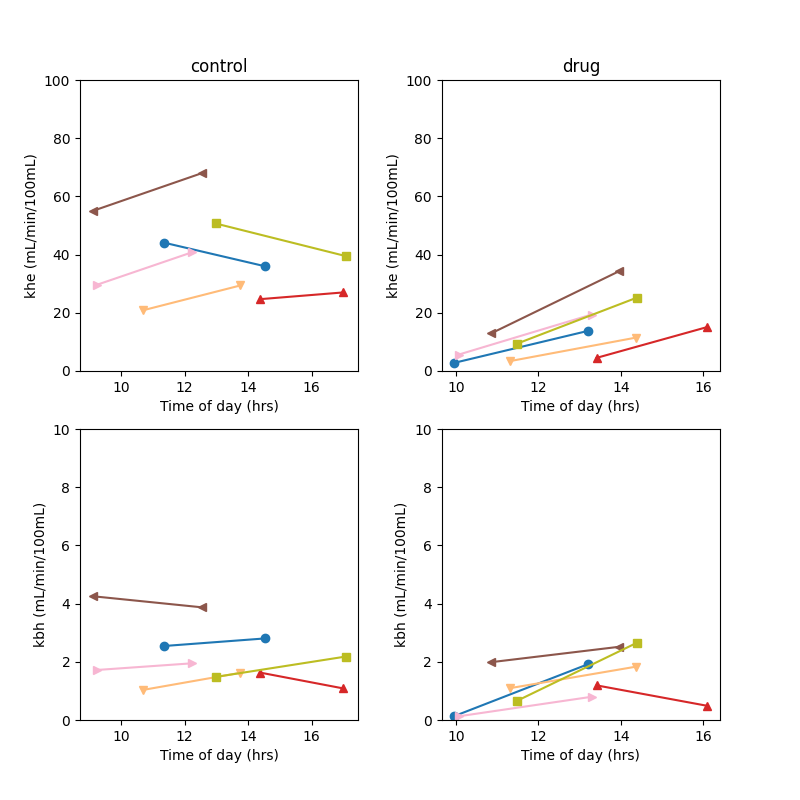
\includegraphics[width=6in]{C:/Users/md1spsx/Documents/GitHub/tristan-human-modelling/build/metformin/results (two scans)/Figures/_diurnal_function.png}%
\caption{Intra{-}day changes in hepatocellular uptake (k\_he, top row) and biliary excretion (k\_bh, bottom row) of gadoxetate at for the control (left column) and treatment (right column). Full lines connect values taken in the same subject at the same day.}%
\end{figure}

%
\end{document}